\lab{Policy Function Iteration}{Policy Function Iteration}
\objective{This section teaches how to improve dynamic programming convergence using policy function iteration.}

Now that we have covered how to solve simple dynamic programming problems by value function iteration, we consider
the convergence of the algorithm.  We demonstrate two additional methods known as policy function iteration, or Howard's
Improvement, and modified policy function iteration.

\section*{Policy Function Iteration}
For infinite horizon dynamic programming problems, it can be shown that value function iteration converges at the
rate $\beta$, where $\beta$ is the discount factor.  In practice, $\beta$ is usually close to one, which means this
algorithm often converges slowly.

In order to examine the value function iteration algorithm, it is helpful to see which functions take the most runtime.
We can perform this analysis using the profiling tools in IPython.
\begin{problem}
\label{prob:profile}
Import your function \li{eatCake} from the Value Function Iteration lab into an IPython environment.
Profile this function with arguments $\beta = .9$, $N = 100$, \li{finite=False}, \li{plot=False}.
Now change the arguments $\beta = .95$ and $N = 1000$.
How does your runtime change? What parts of the code take up the most time?

Recall that we can access the profiling tool in IPython as follows:
\begin{lstlisting}
>>> %prun function_call
\end{lstlisting}
where \li{function_call} is a placeholder for whatever function you wish to profile.
\end{problem}

In Problem \ref{prob:profile} you should have noticed that runtime was significantly longer to run for larger $N$ or
$\beta$ closer to 1.  The profiler gives more detailed information than just the overall runtime, however.
The results of Problem \ref{prob:profile} should look something like the following (we have removed a few
columns and several rows from the full output):
\begin{lstlisting}
     503 function calls in 2.101 seconds

Ordered by: internal time

ncalls  tottime  filename:lineno(function)
    1    1.759   <ipython-input-4-1487b3d35ebf>:1(eatCake)
   59    0.244   {method 'argmax' of 'numpy.ndarray' objects}
    1    0.033   twodim_base.py:427(triu)
    1    0.018   {numpy.core.multiarray.where}
    1    0.009   method 'repeat' of 'numpy.ndarray' objects}
    1    0.009   {method 'outer' of 'numpy.ufunc' objects}
    1    0.005   twodim_base.py:349(tri)
    1    0.004   twodim_base.py:657(mask_indices)
    1    0.004   {method 'astype' of 'numpy.ndarray' objects}
   59    0.004   {method 'reduce' of 'numpy.ufunc' objects}
\end{lstlisting}
We notice that the most time was spent in the maximization step (\li{method 'argmax'}).

Recall that the value function iteration method for the infinite horizon problem
approximates the value function $V$ iteratively, producing a sequence of
approximations $V_1, V_2, V_3, \ldots$ that converge to $V$.
At each step, the algorithm also determines the policy function $\psi_k$
corresponding to the approximated value function $V_k$.
This process can also be viewed as applying the approximate policy function $\psi_k$ once to obtain
the approximate value function $V_k$.
Unfortunately, this gives us a rather crude approximation to the value function,
resulting in slow convergence.

What if instead of iteratively approximating the value function in this manner, we instead iteratively approximate
the policy function, and calculate the exact value function associated with each new policy function?
This is the idea behind the policy function iteration algorithm.
In this way we iterate on the policy functions rather than the value functions.
The algorithm for the policy function iteration can be summarized as follows:
\begin{enumerate}
\item Set an initial policy rule $W' = \psi_0(W)$ and a tolerance $\delta$.

\item \label{item:step2_PFI} Compute the value function assuming this rule is used forever:
\begin{equation*}
V_k(W) = \sum_{t=0}^\infty \beta^t u(W_t - \psi_k(W_t)).
\end{equation*}

\item Determine a new policy $\psi_{k+1}$ so that
\begin{equation*}
\psi_{k+1}(W) = \underset{W'}{\text{argmax}} \{u(W-W') + \beta V_k(W')\}.
\end{equation*}

\item If $\delta_k = ||\psi_{k+1} - \psi_k|| < \delta$, stop, otherwise go back to step \ref{item:step2_PFI} with subscript $k+1$.
\end{enumerate}
In order to compute the value function, $V_k$ corresponding to a given policy $\psi_k$, we must solve
\begin{equation}
\label{Val_Fun}
V_k(W) = u(W-W') + \beta V_k(W')
\end{equation}
for $V_k$.

As always, we take a discrete approximation to $W$, obtaining a length $N$ vector
\[
w = (w_1, w_2, \ldots, w_N)
\]
giving the possible cake quantities.
The variable $W'$ becomes $w' = \psi_k(w)$.
Once we have done this, equation \eqref{Val_Fun} is a linear system which we can rewrite as
\begin{equation*}
V_k(w) = u(w-w') + \beta QV_k(w)
\end{equation*}
where $Q$ is the $N\times N$ matrix
\begin{equation*}
Q_{ij} = \left\{
     \begin{array}{ll}
       1 & \text{if} \quad  w_i' = w_j\\
       0 & \text{otherwise.}
     \end{array}
   \right.
\end{equation*}
Solving this system of equations, we have $V_k(w) = (I-\beta Q)^{-1}u(w-w')$.
Although $Q$ may be large, we can take advantage of the fact that it is sparse, containing only $N$ nonzero entries out of $N^2$ total entries.

\begin{problem}
\label{prob:cake_eating_policyfun}
Solve the infinite horizon cake eating problem from the Value Function Iteration lab again, this time using policy function iteration.
Write a function \li{policyIter} that takes arguments $\beta$ (discount factor), $N$ (size of discrete approximation), and
$W_{max}$ (size of original cake, set to default value of 1). Take the function $u$ to be the square root function, as before.
Return the converged value function and policy function, both of which should be arrays of length $N$.

As in the value function iteration, first create your discrete approximation of the $W$ values:
\begin{lstlisting}
>>> import numpy as np
>>> w = np.linspace(0, Wmax, N)
\end{lstlisting}

You will still need to pre-compute all values of $u(W-W')$, storing these in an $N \times N$ array. Make sure, as before,
that the upper triangular entries are set to large negative values, so that we don't choose to consume more cake than is
available. In the code snippets below, we will refer to this array as \li{U}.

You may also find it convenient to not track the approximated policy function $\psi_k$ directly during the iteration, but
rather to have a length $N$ array \li{psi_ind}, whose $i$-th entry gives the index of $w_i'$ relative to the discrete approximation
$w$. Thus, rather than initializing a policy function $\psi_0$ directly, you can initialize it indirectly by setting, for example,
\begin{lstlisting}
>>> psi_ind = np.arange(N)
\end{lstlisting}
which corresponds to an initial policy $\psi_0(W) = W$.
The policy function vector can be obtained from \li{psi_ind} by simply slicing \li{w} as follows:
\begin{lstlisting}
>>> psi = w[psi_ind]
\end{lstlisting}

In order to take advantage of the sparse matrices $I$ and $Q$, use the following imports from the SciPy \li{sparse} library.
\begin{lstlisting}
>>> from scipy import sparse
>>> from scipy.sparse import linalg
\end{lstlisting}
and the following code to initialize $I$ (outside the loop)
\begin{lstlisting}
>>> I = sparse.identity(N, format='csr')
>>> rows = np.arange(0, N)
\end{lstlisting}
and $Q$ (inside the loop)
\begin{lstlisting}
>>> columns = psi_ind
>>> data = np.ones(N)
>>> Q = sparse.coo_matrix((data, (rows,columns)), shape=(N,N))
>>> Q = Q.tocsr()
\end{lstlisting}
Rather than compute $(I-\beta Q)^{-1}$ directly, use Scipy's sparse solver
\begin{lstlisting}
V = linalg.spsolve(I-beta*Q, u(w-w[psi_ind]))
\end{lstlisting}
where \li{u} is the square root function.

In each iteration, we update \li{psi_indices} much as we did in the value function iteration algorithm:
\begin{lstlisting}
>>> psi_ind = np.argmax(U + beta*V, axis=1)
\end{lstlisting}
where we assume \li{V} has shape \li{(1,N)}.

Use the 2-norm when computing $\|\psi_{k+1} - \psi_k\|$, and set the tolerance to $\delta = 1e-9$.

Take $N = 1000$ and $\beta = .95$.
Plot the policy function and compare with your policy function from the Value Function Iteration Lab, using
the same inputs. You should obtain the same answer, but in less runtime.
\end{problem}

\section*{Modified Policy Function Iteration}
While policy function iteration converges in fewer iterations, solving the linear system can be slow,
especially for problems with a large state space.  There is an alternative to this called modified policy
function iteration.

In modified policy function iteration, we don't compute the exact value function corresponding to a policy.
Instead, at step \ref{item:step2_PFI} of the policy iteration algorithm we iterate $m$ times on the value function
equation \eqref{Val_Fun} to get an approximation of the new value function.  This is faster than solving for the
exact value function for large state spaces.  There is no strict rule on the value of $m$, the number of value function
iterations.  In practice values such as $m=10$ or $m=15$ often work well.

Note that our methods for solving dynamic programs boil down to some combination of two things: iterating on the value
function and iterating on the policy function.  Modified policy function does a combination of the two, taking advantage
of the advantages of both methods.  Because modified policy iteration takes only slightly more work to code than value
function iteration, it is often preferred in practice.  Whether policy or modified policy iteration will perform better
may depend on the problem.

\begin{problem}
Solve the infinite horizon cake eating problem again, this time using the modified policy function
iteration method.

Write a function \li{modPolicyIter} that takes the same arguments as your \li{policyIter} function, along
with an additional keyword argument $m$ (set to default value $m=15$), which gives the number of iterations used
to approximate the value function at each step. Return the converged value function and policy function. 

Much of the code in your \li{policyIter} will be unchanged when implementing this function. The key differences are
as follows.
First, you do not need to initialize the sparse arrays $I$ and $Q$ in the modified policy function iteration.
Secondly, rather than solving a linear system of equations to obtain the value function, you will loop
the equation
\begin{lstlisting}
>>> V = u(w - w[psi_ind]) + beta*V[psi_ind]
\end{lstlisting}
$m$ times in each iteration. Notice how this line of code corresponds with Equation \eqref{Val_Fun}, where
\li{w} represents $W$, \li{w[psi_ind]} represents $W'$, and \li{V[psi_ind]} represents $V(W')$.

The remainder of the code should be unchanged.


\end{problem}

\begin{problem}
Solve the cake eating problem with each of the three methods and report how many iterations each takes.  Use $N= 1000$ as the
number of grid points for $W$ and $\beta = 0.95$.  It is important that you use the same initial guess in each case in order to
make the results comparable.  The accuracy of the initial guess greatly affects the number of iterations to convergence.  Take
your initial guess as $V = 0$, which corresponds to an initial guess of the policy function with indices $[0,1,2,\ldots, N-1]$
(meaning $\psi(W) = W$, i.e. we eat no cake, leaving it all for the next period).
\end{problem}

In general we should see that value function iteration takes more iterations than modified policy function iteration which in turn
takes more iterations than policy function iteration.  It is important to note that this does not directly say anything about runtime.
Each iteration of policy iteration may take longer than an iteration of value function iteration.

\section*{Discrete Choice (Threshold) Problems}\label{SecDiscrChoice}

One powerful application of dynamic programming is that we can make 
models that have both continuous and discrete state variables. These models are sometimes referred to as
discrete choice problems or optimal stopping problems.  Examples include models of employment that involve both
the choice of whether to work and how much to work, models of firm entry and exit that involve the choice of both
whether to produce and how much to produce, and models of marriage that involve the choice of whether to date
(get married or keep dating) and how much to date.
This application illustrates the versatility of dynamic programming as a dynamic solution method

In this lab, we follow a simple version of a standard job search model.
Assume that workers live infinitely long.
We will split a worker's life into discrete time periods, and in each period the worker is either
employed or unemployed, and receives a job offer. The worker must make a choice between discrete actions
(such as accepting or rejecting a job offer), with the goal of maximizing some utility function (hence,
this is a \emph{discrete choice} problem).

We can state this problem in terms of dynamic programming by defining an appropriate value function.
Let the value of entering a period with most recent wage $w$,
current job offer wage $w'$, and employment status $s$ be given by the following value function,
\begin{equation}\label{EqV}
   V(w,w',s) = \begin{cases}
                  V^E(w)    \quad&\text{if}\quad s = E \\
                  V^U(w,w') \quad&\text{if}\quad s = U \\
               \end{cases}
\end{equation}
where employment status is a binary variable $s\in\{E,U\}$ ($E$ indicates ``employed" and $U$ indicates ``unemployed");
a person can be either employed or unemployed.

As in the cake eating problem, the value function is calculated as the sum of some reward (based on the
current state) and the discounted value of entering the next period in some particular state.
The reward function, denoted (as usual) by $u$, gives the utility of spending available funds.
Assuming that a worker receives some wage $x$ in a given period and spends all available money in the period,
the utility of consumption is given by
\[
u(x).
\]
Calculating the value for the next period depends on the employment status in the current period, so we address
this separately for each case.

Let us first consider the case where the individual is unemployed ($s = U$). As is customary, let $s'$ denote the
employment status of the worker in the next period.
In this unemployed state, the worker receives unemployment benefits equal to a fraction of her most recent wage,
i.e. $\alpha w$, where $\alpha \in (0, 1)$.
Hence, the utility of consumption in the current unemployed state is given by
\[
u(\alpha w).
\]

The worker also receives one wage offer ($w'$) per period, and will obtain
this wage in the next period provided that she chooses to accept employment, i.e. provided $s' = E$.
The worker must decide whether to accept the current wage offer $w'$ or to remain unemployed in the next period,
i.e. she must decide on the value of $s'$. How
does she make this choice? She must weigh the value of entering the next period as an employed worker with wage
$w'$ (given by $V^E(w')$) versus the value of entering the next period as an unemployed worker with
previous wage $w$ and unknown wage offer $w''$ (given by $V^U(w,w'')$). Because the worker cannot know
what the future wage offer $w''$ will be, it is treated as a random variable with a particular probability
distribution. Hence, the worker must actually compute the \emph{expected} value of entering the next
period unemployed. This term is simply
\[
\mathbb{E}_{w''}V^U(w,w''),
\]
where $\mathbb{E}_{w''}$ denotes the expectation operator with respect to the probability distribution of future
wage offers $w''$.
To sum up, the worker chooses to accept the wage offer $w'$ or remain unemployed in the next period based on
which option gives the greater expected value, and the value of this decision is given by
\[
\max\Bigl\{V^E(w'), \,\, \mathbb{E}_{w''}V^U(w,w'')\Bigr\}.
\]

The overall value of the current unemployed state with previous wage $w$ and current wage offer $w'$ is
just the utility of consumption plus the discounted value of the next period, i.e.
\begin{equation}\label{EqVu}
V^U(w,w') = u(\alpha w) + \beta \max\Bigl\{V^E(w'), \,\, \mathbb{E}_{w''}V^U(w,w'')\Bigr\},
\end{equation}
where $\beta$ is the discount factor.

Now we turn to the case where the job status is employed ($s = E$).
In this case, the worker receives a wage $w$ in the current period, and so the utility of consumption is
just
\[
u(w).
\]
In the next period, the worker will have most recent wage $w$, she will receive wage offer $w''$, and will
have employment status $s'$. As in the unemployed case, $w''$ is unknown and treated as a random variable.
Unlike the unemployed case, however, the worker's future employment status $s'$ is not under her control,
but rather is also a random variable. The reason for this is that the worker will remain employed
until she loses the job, a random event that occurs with some fixed probability in each time period.
Hence, we must calculate the expected value of the next period with respect to both $w''$ and $s'$.
We may write the entire value function for the employed case as
\begin{equation}\label{EqVe1}
   V^E(w) = u(w) + \beta \mathbb{E}_{w'',s'}V(w,w'',s').
\end{equation}

To calculate the expectation term, we need to know the joint probability distribution over $w''$ and $s'$.
This can be characterized in the following way.
We assume that $s'$ and $w''$ are independent. Hence, we can split the joint expectation
operator into the composition of the two individual expectation operators:
\[
\mathbb{E}_{w'',s'} = \mathbb{E}_{w''}\mathbb{E}_{s'}.
\]
Let $\gamma$ represent the probability that an employed worker becomes unemployed in the next period,
so that $1-\gamma$ is the probability of remaining employed in the next period.
If the worker stays employed in the next period ($s' = E$), then next period's wage equals the current
period's wage, and the term inside the expectation is
\[
V(w,w'',E) = V^E(w).
\]
We then have
\begin{align*}
\mathbb{E}_{s'}V(w,w'',s') &= (1-\gamma)V(w,w'',E) + \gamma V(w,w'',U)\\
&= (1-\gamma)V^E(w) + \gamma V^U(w,w'').
\end{align*}
Notice that the term $(1-\gamma)V^E(w)$ is constant with respect to $w''$. Then
\begin{align*}
\mathbb{E}_{w''}\mathbb{E}_{s'}V(w,w'',s') &= \mathbb{E}_{w''}\left[(1-\gamma)V^E(w) + \gamma V^U(w,w'')\right]\\
&= \mathbb{E}_{w''}(1-\gamma)V^E(w) + \mathbb{E}_{w''}\gamma V^U(w,w'')\\
&= (1-\gamma)V^E(w) + \gamma \mathbb{E}_{w''}V^U(w,w'').
\end{align*}
Hence, we can rewrite \eqref{EqVe1} as follows:
\begin{equation}\label{EqVe2}
   V^E(w) = u(w) + \beta \Bigl[(1-\gamma)V^E(w) + \gamma \mathbb{E}_{w''}V^U(w,w'')\Bigr].
\end{equation}

We have now completely described the value function. What about the policy function?
The policy function for the unemployed worker gives her decision on whether to accept the job $s'=E$
or to reject the job $s'= U$.
This will be a function of both the most recent wage $w$ and the current wage offer $w'$.
The employment status $s'$ in the next period is determined by the policy function $\psi$:
\[
s' = \psi(w,w').
\]

These discrete choice problems are often called threshold
problems because the policy choice depends on whether the state variable is greater than or less than
some threshold level. That is, an unemployed worker will accept a job if and only if the offer wage is
above some set amount that depends on the most recent wage $w$. In the labor search model,
the threshold level is called the ``reservation wage'' $w_R'$. The reservation wage $w_R'$ is defined as
the wage offer such that the worker is indifferent between accepting the job $s' = E$ and
staying unemployed $s' = U$. Hence, this reservation wage satisfies the equation
\begin{equation}\label{EqWR}
   V^E(w_R') = E_{w''}\left[V^U(w,w'')\right].
\end{equation}
The policy function will then take the form of accepting the job if $w' \geq w_R'$ or
rejecting the job offer and remaining unemployed if $w' < w_R'$:
\begin{equation}\label{EqSprime}
   s' = \psi(w,w') = \begin{cases}
                      E \quad\text{if}\quad w' \geq w_R' \\
                      U \quad\text{if}\quad w' < w_R'.
                   \end{cases}
\end{equation}
Figure \ref{fig:disc_policy} shows an example of the discrete policy function.

\begin{figure}
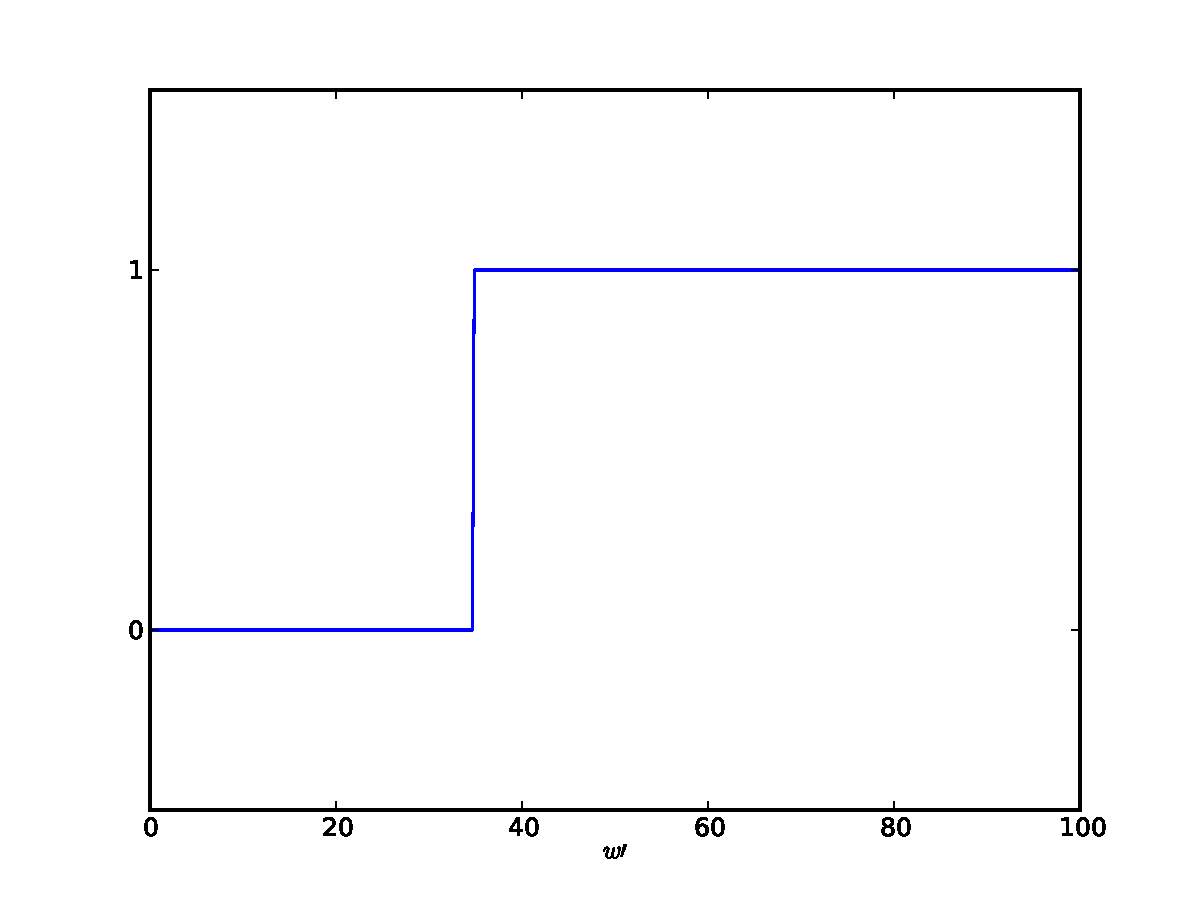
\includegraphics[width=\textwidth]{disc_policy.pdf}
\caption{Here is the policy function for fixed $w = 50$.  Numerically we let 0 represent unemployment, $U$,
and 1 represent employment, $E$.  Thus we see that an individual will choose to take a new job, given
their old wage was 50, at a wage of roughly 35.  Thus for a previous wage of 50, we say the reservation wage is 35.}
\label{fig:disc_policy}
\end{figure}

In summary, the labor search discrete choice problem is characterized by the value functions \eqref{EqV}, \eqref{EqVu},
and \eqref{EqVe2}, the reservation wage \eqref{EqWR}, and the policy function \eqref{EqSprime}. Because wage offers
are distributed according to some given probability distribution (denote the cdf by $F(w')$),
and because the policy function takes the form of \eqref{EqSprime},
the probability that the unemployed worker receives a wage offer that she will reject is $F(w_R')$ and the probability
that she receives a wage offer that she will accept is $1 - F(w_R')$. Just like the continuous-choice cake eating
problems, this problem can be solved by value function, policy function, or modified policy function iteration.

The value function iteration solution method for the equilibrium in the labor search problem is analogous to the
value function iteration from the previous labs. The only difference is that two value functions ($V^E$ and $V^U$)
must converge to a fixed point in this problem instead of just one value function converging in the previous problems.
Although there are two value functions to consider, there is only one policy function, since decisions are only made
in the unemployed state.  Thus, there is only one policy function on which to iterate in the case of policy or modified
policy iteration.

In the following problems, you will solve the job search problem using value function iteration and modified policy
function iteration. Assume that the consumption utility function $u$ is given by
\[
u(w) = \sqrt{w}.
\]
Assume that the probability of becoming unemployed in a given period is $\gamma = 0.10$, the fraction of wages paid
in unemployment benefits is $\alpha = 0.5$, and the discount factor is $\beta = 0.9$.

Assume that the log of wage offers are distributed normally.  We then say that offers are distributed
lognormally and write
\[
w'\sim \text{LogN}(\mu,\sigma).
\]
This is a convenient choice for the distribution of
wage offers.  Among other things, it guarantees that wage offers will be positive.
A mean of $20$ and variance of $200$ are typical parameters of such a wage distribution,
and we will use these parameters in the following problems.

As usual when dealing with continuous variables, we form a discrete approximation of
the possible wage values. In particular, approximate the wage values by a vector of
length $N = 500$ of equally-spaced values from $w_{min} = 0$ to $w_{max} = 100$, inclusive.
We then form a corresponding discrete approximation of the probability density function
$f(w')$ for the lognormal wage offers using code provided in the file \li{discretelognorm.py},
as follows, where \li{w} is the length-$N$ vector of wage values, $m$ is the mean, and $v$ is
the variance as specified above:
\begin{lstlisting}
>>> from discretelognorm import discretelognorm
>>> f = discretelognorm(w, m, v)
\end{lstlisting}
The function \li{discretelognorm} computes the discrete pdf of the specified lognormal distribution in much
the same way that you calculate the discrete normal pdf when solving the stochastic cake eating problem.


\begin{problem}
Solve the job search problem using value function iteration. Return the converged value functions
$V^E$ and $V^U$, as well as the converged policy function $\psi$. The following steps provide detailed
instructions. Note that there are multiple ways to proceed, and the following is simply one (fairly good)
possibility.
\begin{enumerate}

   \item As described above, represent the possible wage values by an array \li{w} of length
   $N$. Denote this array entrywise by
   \[
   w = (w_1,w_2,\ldots,w_N).
   \]
   Calculate the corresponding discrete lognormal pdf \li{f}, exactly as shown above.

   \item Note that $u(w)$ and $u(\alpha w)$ are needed when computing the value functions.
   Since these quantities do not change from one iteration to another, it is smart to
   compute them once at the outset. Denote $u(w)$ by \li{uw} and $u(\alpha w)$ by \li{uaw}.
   These are easily calculated as follows:
\begin{lstlisting}
>>> uw = u(w)
>>> uaw = u(alpha*w).reshape((N,1))
\end{lstlisting}
    where \li{u} is the square root function. We must reshape \li{uaw} because of array broadcasting
    issues that arise in the code snippets below.

   \item Since $V^E$ is a function of only $w$, it will be represented by a vector of length $N$, where
   the $i$-th entry gives $V^E(w_i)$. The unemployed value function $V^U$, however,
   is a function of both $w$ and $w'$, so it will be represented by an $N \times N$ array,
   where the $(i,j)$-th entry gives $V^U(w_i,w_j)$. Initialize the entries of these arrays to 0:
\begin{lstlisting}
>>> VE = np.zeros(N)        #employed value function
>>> VU = np.zeros((N,N))    #unemployed value function
\end{lstlisting}

   \item Note that $\mathbb{E}_{w''}V^U(w,w'')$  is needed to calculate both $V^E$ and $V^U$.
   This expectation depends on $w$, and so can be represented by a length $N$ array, where the
   $i$-th entry is $\mathbb{E}_{w''}V^U(w_i,w'')$.
   It is convenient to assign a variable to this array to keep track of it throughout the iterations.
   We denote the expectation by \li{EVU}, and initialize it to zeros:
\begin{lstlisting}
>>> EVU = np.zeros(N)
\end{lstlisting}

   \item For reasons that will soon become apparent, we will need to create an $N\times N$ helper array
   whose rows are equal to \li{VE} (call this array \li{MVE}), and a $N \times N$ helper array whose columns
   are equal to \li{EVU} (call this array \li{MEVU}).
   At the outset, simply initialize these arrays to zeros.

   \item Because job status is a binary variable, the policy function returns one of two possible values. It is
   convenient to represent ``employed" by $1$ and ``unemployed" by $0$. Now the policy function depends
   on $w$ and $w'$, so it will also be represented by an $N\times N$ array \li{PSI} of zeros and ones,
   where the $(i,j)$-th entry gives $\psi(w_i, w_j)$.

   \item Now we are ready to begin the iteration.
   A single iteration involves computing the updated value functions $V^E$ and $V^U$ from
   equations \eqref{EqVe2} and \eqref{EqVu} and then calculating the $2$-norm distance between
   both pairs of old and updated value functions to test for convergence. If both of these
   $2$-norm distances are less than $10^{-9}$, terminate the iteration.

   Before calculating the updated value functions, we first update our helper arrays \li{MVE} and
   \li{MEVU}. The rows of \li{MVE} need to equal \li{VE}. We can use array broadcasting:
\begin{lstlisting}
>>> MVE[:,:] = VE.reshape((1,N))
\end{lstlisting}
   The columns of \li{MEVU} need to equal \li{EVU}, so use a similar technique:
\begin{lstlisting}
>>> MEVU[:,:] = EVU.reshape((N,1))
\end{lstlisting}

   Now let us address how to compute the updated $V^U$, which we denote by \li{VU1}.
   Equation \eqref{EqVu} shows that it is the sum of
   two terms. The first, $u(\alpha w)$, we have already computed and stored in the variable \li{uaw}.
   The second term involves a maximization between two alternatives. One can imagine writing
   a double for loop ranging over the values of $w'$ and $w$ to compute each individual
   $\max\{V^E(w'), \mathbb{E}_{w''}V^U(w,w'')\}$, but we can take advantage of the helper
   arrays \li{MVE} and \li{MEVU} to do this computation in one efficient line of code.
   Note that the $(i,j)$-th entry of \li{MVE} is just $V^E(w_j)$ and the $(i,j)$-th
   entry of \li{MEVU} is $\mathbb{E}_{w''}(w_i, w'')$, and
   \[
   V^U(w_i,w_j) = u(\alpha w_i) + \beta\max\{V^E(w_j), \mathbb{E}_{w''}V^U(w_i,w'')\}.
   \]
   Hence, taking the entrywise maximum of the arrays \li{MVE} and \li{MEVU} gives us the appropriate
   max term for $V^U$. To get the entrywise maximum of two arrays, stack the arrays along a new
   axis using \li{np.dstack}, and maximize along that axis. The computation for \li{VU}, then, is
   \begin{lstlisting}
>>> VU1 = uaw + beta*np.max(np.dstack([MEVU, MVE]), axis=2)
   \end{lstlisting}

   Calculating the updated $V^E$, denoted by \li{VE1}, is more straightforward.
   Equation \eqref{EqVe2} shows that it is just
   a particular linear combination of the arrays \li{uw}, \li{VE}, and \li{EVU}:
   \begin{lstlisting}
>>> VE1 = uw + beta*((1-gamma)*VE + gamma*EVU)
   \end{lstlisting}

   We can now calculate the 2-norm distances between old and updated value functions.
   It remains to update \li{VE}, \li{VU}, and \li{EVU}.
   The first two updates are trivial, and calculating \li{EVU} is equivalent to the
   matrix-vector multiplication of \li{VU} with \li{f}. This is similar to how we computed
   expectations in previous labs:
   \begin{lstlisting}
>>> EVU = np.dot(VU,f).ravel()
   \end{lstlisting}
   We use the \li{ravel} function to ensure that \li{EVU} is a flat array.

   \item Notice that it is not necessary to iteratively update the policy function, as it is not needed
   to update the value functions. Thus, we need only compute the policy function once, after convergence
   of the value functions has been achieved. This is done in a manner similar to calculating
   $\max\{V^E(w'), \mathbb{E}_{w''}V^U(w,w'')\}$ as described above, except we need to take the \emph{argmax}:
\begin{lstlisting}
>>> PSI = np.argmax(np.dstack([MEVU,MVE]), axis=2)
\end{lstlisting}

   \item Compute the reservation wage $w_R'$ as a function of the current wage $w$. It will be represented
   by a length $N$ array called \li{wr}. The reservation wage is the
   value of $w'$ where the policy function changes from zeros to ones (the optimal choice changes from remaining
   unemployed to accepting the job offer). We can calculate this as follows:
   \begin{lstlisting}
>>> wr_ind = np.argmax(np.diff(PSI), axis = 1)
>>> wr = w[wr_ind]
   \end{lstlisting}

   \item Plot the equilibrium reservation wage $w_R'$ of the converged problem as a function of the current
   wage $w$ with the current wage on the $x$-axis and the reservation wage $w_R'$ on the $y$-axis. This is
   the most common way to plot discrete choice policy functions. The reservation wage represents the wage
   that makes the unemployed worker indifferent between taking a job offer and rejecting it. So any wage
   above the reservation wage line represents $s' = E$ and any wage below the reservation wage line represents
   $s' = U$. Your plot should resemble that in Figure \ref{fig:res_wage}.

\end{enumerate}
\end{problem}

\begin{figure}
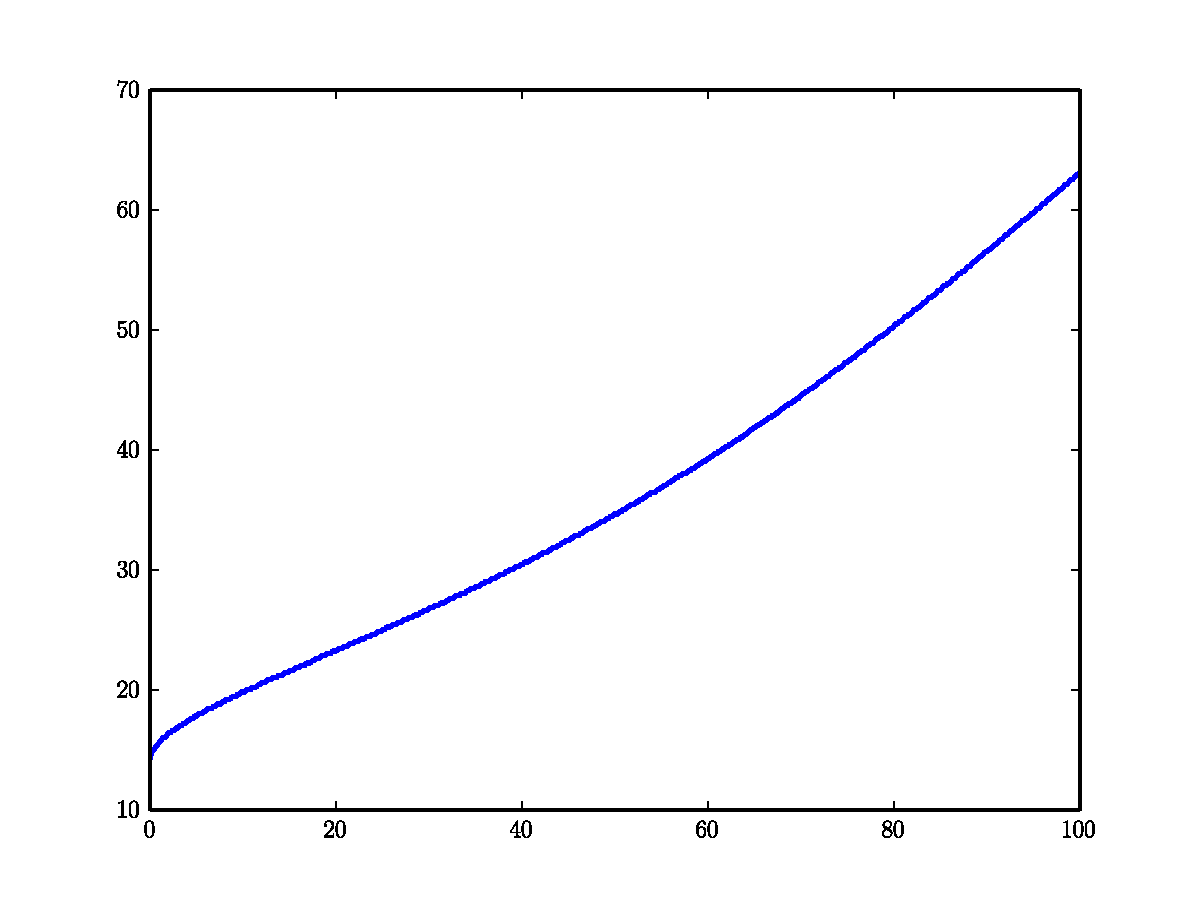
\includegraphics[width=\textwidth]{reservation_wage.pdf}
\caption{The reservation wage as a function of previous wage for the job search problem.}
\label{fig:res_wage}
\end{figure}

In the previous problem, it was necessary to iterate on two value functions.
Consequently the convergence is relatively slow.
We can improve upon this situation by using modified policy function iteration.

\begin{problem}
Solve the same problem, this time using modified policy function iteration with $15$ value function iterations
within each policy iteration.  You should be able to re-use much of your code from the previous problem.

Start off by initializing all of the same variables. Additionally, initialize your policy function array \li{PSI},
say
\begin{lstlisting}
>>> PSI = 2*np.ones((N,N))
\end{lstlisting}

Next comes the iteration.
Essentially, the iteration will consist of an outer while-loop (which terminates once the 2-norm distance
between successive policy functions passes below $10^{-9}$), and an inner for loop (with $15$ loops).


The first step in the while-loop is to calculate the new policy function \li{PSI1}, just as in the previous
problem. Next, perform the inner for-loop, which consists simply of the value function iteration, but this
time using the current policy function. This means the line of code
\begin{lstlisting}
>>> VU = uaw + beta*np.max(np.dstack([MEVU, MVE]), axis=2)
\end{lstlisting}
is no longer valid, as it does not use the policy function. We must instead have
\begin{lstlisting}
>>> VU = uaw + beta*(MVE*PSI1 + MEVU*(1 - PSI1))
\end{lstlisting}
Why is this code correct?

Finally, after exiting the for loop, calculate the 2-norm distance between the old and the new policy function,
and then update your old policy function, i.e.
\begin{lstlisting}
>>> PSI = PSI1
\end{lstlisting}

After convergence is achieved, once again compute the reservation wage array, and plot it as in the previous
problem. Then return the converged policy function.
\end{problem}

\begin{problem}
How many iterations did the value function iteration method take?
How many iterations did the modified policy function iteration method take?
Which was faster?
\end{problem}
